\chapter{Implementation Details}

\section{Case of study 1: Cluster and Honeypot for a Ransomware attack}

\subsection{Workflow}

After a first phase of research related to honeypots, their taxonomy and features, the work shifted to an actual implementation of at least one of the use cases. In this section the use case regarding a malware honeypot is tackled.\\
In the very first days, the idea was to consider 4 ESP32 devices as nodes in the cluster. ESP32 is a brilliant device due to its low cost but it lacks some of the features needed for this project, such as a reasonable memory capacity to store enough data files.\\
Therefore, the second option consists in using 4 Raspberry Pi devices due to their memory storage, way wider than ESP32.\\
Once the OS, a lighter distribution of Linux released for Raspberry, got mounted, the actual development started.\\
At first, a Python script to build a randomly generated file system got released ("createProductionFiles.py"). This script only generates production files and not sentinel files.\\
Then, a new Python script ("createSentinels.py") was used to generate sentinel files and spread them across the file system.\\
For each Raspberry, two scripts ("NEWNEWpubsub.py" and "rpiClient.py") provide MQTT and monitoring functionalities.\\
The last phase of the project focused on the deployment of ransomware to test the defensive mechanism. Literature shows examples of ransomware that can be generated thanks to PowerShell commands, but the final choice was to create an ad-hoc ransomware thanks to a further Python script ("rpiClientPubOnly.py").\\
The first idea regarding the defensive mechanism was to develop a honeypot on one of the machines in the cluster. This could make all other nodes way simpler and they should only perform functional tasks, exempting them from performing security tasks. On the other hand, if any attack targets the honeypot, then security over the whole cluster is compromised.\\
The current implementation includes a different solution based on a distributed honeypot in the cluster: each node both performs functional and security tasks. If a node is offline, other nodes will still perform honeypot tasks and security is not compromised.


\subsection{Structure of the IoT cluster and cluster functionalities}

As previously mentioned, the cluster shows a fully connected mesh topology thanks to which each node can communicate to any other in the cluster. This is posssible thanks to MQTT, a communication protocol based on the publish/subscribe paradigm. A node can be a publisher, a subscriber or even both kinds of entities. MQTT is one of the most popular protocols in IoT due to its light header overhead and broadcast features. Subscriber nodes subscribe to a topic and whenever a publisher node communicates a message in the network with the very same topic, such subscribers are able to collect it. A drawback of this approach is the presence of a message broker in the middle of each peer to peer communication. A message broker is an entity, external to the cluster, that receives messages by publishers and forwards them to subscribers. In the case of this project, the message broker is hosted by test.mosquitto.org.\\
Messages exchanged in the cluster can be of two kinds, with the possibility to extend to further kinds:

\begin{itemize}
  \item Commands. They represent the functional aspect of the cluster taken into account. Normally such messages should be published by the dispatcher in the cluster but it is also possible to assume that in a load balancing cluster a node overloaded with work can delegate another node to perform some of the tasks, thus sending a bash command via MQTT message. This is clearly a vulnerability of the cluster, that the ransomware will try to exploit.\\
This kind of message shows the following structure, in JSON: \{"src" : <publisher\_ID>, "dest" : <dest\_node\_ID>, "command" : <command>\}. The topic is "PoliTo/C4ES/<dest\_node\_ID>/command".\\
It is important to notice that any command dispatched to any of the machine is logged in a text file, "log.txt". This feature is compliant to the research purposes of a malware honeypot, that lets the malware move freely in a confined space and records its behavior both for research purposes and for improving security thanks to newly collected information;
  \item Attack notifications. A node (hereafter referred to as "victim" node) will broadcast a message of this kind if the periodic check on sentinel files fails. All other nodes in the cluster collect this message and will insert the victim node to their own internal blacklist because the victim's messages are no longer considered reliable, since an infection is in progress. The victim is deleted from the blacklist aftter a fixed amount of time.
This kind of message shows the following structure, in JSON: \{"hash\_mismatch\_in" : <sentinel\_file\_path>, "untrust\_topic" : <victim\_node\_pubTopic>\}. The topic is "PoliTo/C4ES/<victim\_node\_ID>/attack".
\end{itemize}


\subsection{Creation of File System}

Production files are files that contain useful data to be elaborated in the cluster. An example could be data gathered from sensors spread in a wide area that are then all forwarded to the nodes in the cluster for some post processing operation. Such post processing operations could be too complex to be performed on the edge by sensor nodes. For instance, you could think of some FIR filters that cut out sensed measures that show too much difference with respect to recent values (it is the case for analog sensed measures, such as temperature).\\
In this version of the project, production files are filled with random content since nobody will ever operate on data. The file system is filled, in every directory, with a variable number of production files thanks to "createProductionFiles.py".\\
Sentinel files, on the other hand, are deployed with the sole purpose of being tripwires for an attacker. Their content, in this version of the project, is also randomly generated. They should always appear on top and bottom of the list of files displayed in a directory. This feature got implemented by ordering production files alphabetically, extracting the first and the last file names and finding names for sentinels (thanks to the ASCII table) such that they would get over the first and last production files. For example, if alphabetically the first and last production files are named "aProductionFile.txt" and "zProductionFile.txt", then two sentinels are named "0aProductionFile.txt" and "zQroductionFile.txt" respectively.\\
Other sentinels are deployed in the same directory, in the middle of production files, thanks to a logic based on ASCII as well. This system does not aim at filling up the file system with sentinels. On the other hand, its goal is to place them in a smart way. The number of sentinels is proportional to the number of production files, in a 1:3 ratio.\\
Placing a sentinel at the bottom of the files list is crucial for preventing malicious actions by the malware. If the malware understands that sentinel files are present, a trivial way to avoid encountering sentinel files could be simply reversing the displayed list of files.\\
Once a sentinel file is created, its hash digest and name are stored in a file, in the very same directory, called ".hashes.txt". This file, once the sentinels are all created, is set in READONLY mode and stores the original hash values for the integrity check on sentinels.\\
This is a case in which we consider the command "chmod" as our root of trust.\\


\subsection{Monitoring Phase}

Integrity is the cybersecurity property according to which the content of a file or a message should not change in an undesired manner with respect to the legitimate parties involved in the management of the message or file itself.\\
Checking the content of all sentinel files in the file system is an operation that is too expensive due to the high time of computation. Moreover, it is a cost that depends linearly on the size of the file to check.\\
Hash digests provide a simple, yet reliable, way to check the integrity of a file by simply asserting that its hash digest is the same as the one previously stored and kept safe. This is a reasonable statement as long as the original hash digests are kept away from attacks and the hash algorithm cannot be cracked in short time. A way to crack hash algorithms relies on finding a collision. A collision is a couple of plaintext messages that both lead to the same digest. Hash algorithms create a "summary" of the content of a file or message, thus they are always collision prone. SHA512 got chosen as hash algorithm thanks to its strong collision resistance properties.\\  
Integrity check of sentinel files is performed periodically on each raspberry in the cluster. For each directory in the file system, the file ".hashes.txt" is read. For each sentinel present in the file, the hash digest is recomputed by means of SHA512 and matched against the stored hash. If a mismatch occurs in any of the sentinel files, then the raspberry (i.e., the victim of the attack) will perform two operations:

\begin{enumerate}
  \item An attack notification is broadcasted to all nodes in the cluster, which will no longer consider the victim as reliable;
  \item An immediate shutdown is performed, breaking any possible encryption operation. In the current release, a technician is supposed to restore the status of the victim raspberry, by switching it on again within a fixed amount of time. Once this amount of time has elapsed, the victim node is considered reliable again.
\end{enumerate}


\subsection{Ransomware}

As previously mentioned, an adoption of a real ransomware got discarded. However, the ad-hoc ransomware shows all the significant operations that a real one would perform.\\
Also, some enhanced attack features are taken into account. For instance, we supposed that once a ransomware is in the victim's system it might understand that some tripwire files are placed (since it is a well known technique) and therefore might perform some files reordering. Files reordering could arrange files in a way such that production files could be encountered first, compromising the defensive mechanism. Such an arrangement is not possible in our solution since a masking of some bash commands is performed, not allowing harmful commands such as "sort -r" that would order files in a random way, in a given directory. Command redirection is tackled in the next section of this chapter.\\
In this cluster structure, the vulnerability that could be exploited by the ransomware is that there is no clear dispatching device to give commands. The ransomware could claim to be a node sending commands legitimately.\\
The ransomware performs four main operations:

\begin{enumerate}
  \item A pair of asymmetric RSA keys is generated on its own system;
  \item The public key is injected by means of a MQTT message to the victim's system, that has no means to deny the passage of the file;
  \item The public key is imported by the victim because the ransomware dispatches a "gpg --import publicKey" command;
  \item The encryption is performed recursively on the whole file system using the public key just injected. This means that the only way to recover files is to collect the private key owned by the ransomware.
\end{enumerate}


\subsection{Command Redirection}

EDWARD


\section{Case of study 2: Cluster and Honeypot for a DoS attack}
\subsection{Instruments used and workflow}
In order to simulate our IoT cluster with the honeypot, we decide to implement a simulation using python. The most important aspect 
to respect when developing a client-server application, like our ioT cluster, is that the servers and the sensors have to be able to exchange data 
with each other. The module sockets present in the python library allow us to support networking protocols between two or more processes across machines. 
In this particular case, we use TCP sockets, where on one side a process acts like a client and on the other side a process act like a server.
 Also, python offers module selectors that allow us to serve multiple socket connections. In particular the .select() method allows us to check for I/O completion on more than one socket. So we can call .select() to see which sockets have I/O
 ready for reading and/or writing.  We also want to underline that with .select()  we’re not able to run concurrently. 
Regarding the workflow, we started with an example of scripts for client and server. Then we develop a theoretical model for the sensors, in this particular 
implementation we focus on terminal and door. Then we test it with a server that could handle multiple connections. Then we develop the honeypot, first that handles only 
one request of checking the new connection, then that could work with multiple connections. Than we create an IPS that could interact with sensors, server and the honeypot. 
After we transform the IPS into a simple dispatcher. In the last, we run the scripts and see if together can work correctly.  
\subsection{ First structure of the IoT cluster}
In our first simulation we decided to implement an high-interaction honeypot and a cluster reported in the figure below.
\begin{figure}[h!]
  \centering
  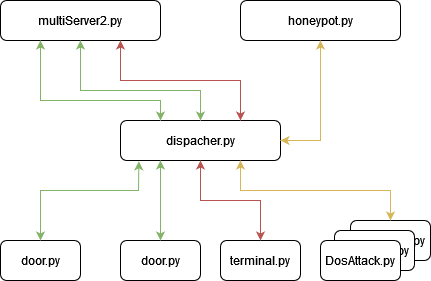
\includegraphics[width = 12cm]{images/HighInterationHoneypot.drawio.png}
  \caption{Our simple IoT cluster with an high-interaction honeypot}
  \label{fig:DosImpl1}
\end{figure}
\FloatBarrier
\noindent
We have different type of client (just like in the reality of an heterogeneous IoT cluster).
In the nexts subsections we will explain the purpose of every script and how they interact. We would like to remind that on the git repository there is also a tutorial about the use of the first version of the cluster.
\subsection{Door.py}
This script represent a door that could be controlled by our system. It have a global variable named status , that could assume 2 values, UNLOCK and LOCK.
This are the status of the door. When the "sensor" is turned on,  it send 2 packets to the server with the initial status of the door, then it wait for commands from the server.  The packets send by the door sensor have this format: "topic: DOOR data: LOCK/UNLOCK IPFALSE: 129.0.0.1". The IPFALSE filed was an attempt
to mask the loopbacks IP with external IP, but then we understand that this was not necessary. A socket can be distinguished by another by the couple (IP,port) 
of the client and the server. When the scripts from this implementation will be launch from different network, the system will behave in the same way of  our tests on loopback. We decided to leave this field because if in the future we need to exchange more data, we could recycle it, of course changhing the name.
The data that the door could receive from the server have this format: "topic: SERVER data: STATUS/LOCK/UNLOCK IPFALSE: someData". When the server 
request the status, the door check the variable STATUS and sent it value to the server.  If the command is LOCK the STATUS variable is set to LOCK, if the command is UNLOCK the STATUS variable is set to UNLOCK.


\subsection{terminal.py}
This script represent a terminal where the admin of the IoT cluster could control the sensors. The terminal offer a set of command , that we report here.
\begin{itemize}
\item \textbf{LISTD}: it return the number of door connected to the system, it do not require other argument. In our system to refer a specific door we use a number to identify it. So if 2 doors are connected to the server, to act on the first door we digit 1, to act on the second we digit 2, to act on all trhe doors we digit ALL. The format for the packes from the terminal to the server for this command is :"topic: TERMINAL data: LISTD data2: bho IPFALSE: 130.0.0.1". The field data2 is used by the other commands
\item \textbf{OPEND}: it allow the user to open a specific door connected to the system or open all the doors. For example, if we want to open only the door 2 we digit OPEND 2, if we want to open all the doors we digit OPEND ALL .  The format for the packes from the terminal to the server for this command is :"topic: TERMINAL data: OPEND data2: 1/2/ecc../ALL IPFALSE: 130.0.0.1".
\item \textbf{CLOSED}: it allow the user to close a specific door connected to the sytem or close all the doors. For example, if we want to close only the door 2 we digit CLOSED 2, if we want to close all the doors we digit CLOSED ALL .  The format for the packes from the terminal to the server for this command is :"topic: TERMINAL data: CLOSED data2: 1/2/ecc../ALL IPFALSE: 130.0.0.1".
\item \textbf{GETSTATUSD}: it allow the user to know the status of all the doors connected to the system. The format for the packes from the terminal to the server for this command is :"topic: TERMINAL data: GETSTATUSD data2: 1/2/ecc../ALL IPFALSE: 130.0.0.1". We could check the status of a specific door or of all the doors. 
\end{itemize}
After a coomand is sent to the server, our terminal start waiting for the response. The returned data depends from the command wrote to the server.
\begin{itemize}
\item \textbf{data for LISTD}: the data format returned by the server is : "topic: SERVER data: LISTD data2: 'NumberOfPortConnected' IPFALSE: 128.0.0.1" . Thew termianl print the number of door available.
\item \textbf{OPEND}: the data format returned by the server is : "topic: SERVER data: OPEND data2: 'statusOfTheDoor' IPFALSE: 128.0.0.1" . The terminal then show the status of the door selected or off all the door selected
\item \textbf{CLOSED}: the data format returned by the server is : "topic: SERVER data: CLOSED data2: 'statusOfTheDoor' IPFALSE: 128.0.0.1" . The terminal then show the status of the door selected or off all the door selected
\item \textbf{GETSTATUSD}:  the data format returned by the server is : "topic: SERVER data: GETSTATUSD data2: IDDoor\_statusDoor IPFALSE: 128.0.0.1" . The terminal then show the status of the door selected or of all the door selected .
\end{itemize}
As it is implemented, if the termianl do not receive a response from the server, it stops working.  In future version we could add a timer, and after some time elapsed, we stop wainting from the response and rise an error.


\subsection{dispacher.py}
The dispacher is the first line of defense controlled by our honeypot. All the new connection from outside the network are sent to the dispacher. Here we have 3 list in python, one for the trusted socket named socketWhiteList, that could communicate with the server. Every socket in the white list have a personal socket from the dispacher to the server, the couple is saved in the list coppiaSocketWhiteListSocketServer. The list socketPending save all the new connection from outside that are waiting from the response of the honeypot. When a new connection arrive to the dispacher, the packet sent are redirect to the honeypot. The packet from the dispacher to the honeypot are sent in the same socket named socket\_honey. When a response from the honeypot arrive, if the connection is approved the dispacher move the socket from the list of the pending one to the list of the whitesocket. If the connection is not approved the sockert is delete from the list of the pending one and closed forever.  When a new connection arrive, the dispache sent to the honeypot first the peer name of the new connection, and then the first packet received from it. While a connection is pending, all the other packets from outside are lost, it's just an implementation choise.

\subsection{DosAttack.py}
The script for the Dos attack is very simple,  after establish a connection it start send random data using the socket. 


\subsection{honeypot.py}
The honeypot control the packets from the new connection fro the outside to the dispacher. If the came from a terminal or a door, the new connection is approved , otherwise is not approved. The format of the data from the honeypot to the dispacher is:"ip-port: (ip, port) status: TRUSTED/UNTRUSTED" . The honeypot receive from every connection to check 2 data, the peer name that will be saved and then resent to the dispacher to specify what connection the honeypot is refeiring, and the packet to analyze. 

\subsection{multiServer2.py}
The server have to handle all the connection of the sensors. It have to connect the terminal to the doors, and send the command from the terminal to the correct door. If the command is for all the doors connected, it send a packet with the command to all of them. It have a list of sockets of the doors and a list for the socket of the terminals. As it is implemented, our system work with only one terminal connected to the server, but this could be ealisy changed. The server have to nìbe reached only by the packtes from the dispacher. 

\subsection{How to start the scripts}
In order tro run the simulation in the correct way, we need first to launch the honeypot, with the command \textbf{python honeypot.py 127.0.0.2 65430}. The last 2 argument are the Ip and the port number. They are just an example , but it must be the same of the values saved in the dispacher.py in the global variable HOST\_H and PORT\_H . Then we start the server with the command  \textbf{python multiServer2.py 127.0.0.3 65429}, with the argument equal to the value HOST\_S and PORT\_S in the dispacher. Then we launch the dispacher with the command  \textbf{python dispacher.py 127.0.0.1 65430} . Then we could start all the sensors, in order to connect then to the dispacher, the global variable in all the sensors and Dos Attack HOST and PORT must be the same of the argument given to the dispacher. 

\subsection{ Second structure of the IoT cluster}
After the presentation of our projects it was notice to our group that the honeypot and the dispacher could be collapsed in just one "server" , actualy a script, that handle all the function of the dispacher and the honeypot.  So we create the script dispacherAndPot.py . Here, we have a function named honeypot, that , like the reader probably already iìunderstand, is the honeypot. When a new connection arrive, this function is called and check the packets sent to the dispacher. If it is ok it return 1, otherwise 0. This low-interaction is much more efficient and simple, it do not lose packet from pending connection and we do not neeed to create socket between the honeypot and the dispacher. According to the complexity of the simulation right now, this implementation is much better, but if we want for example to improve the honeypot with new feature, like the ones from our other implementation, we suggest to use the first version. The picture below report the structure of the second implementation. 
\begin{figure}[h!]
  \centering
  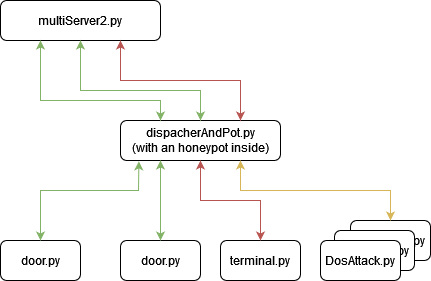
\includegraphics[width = 12cm]{images/lowInterationHoneypot.drawio.png}
  \caption{Our simple IoT cluster with a low-interaction honeypot}
  \label{fig:DosImpl2}
\end{figure}
\FloatBarrier
\noindent











%cancella
This is where you explain what you have implemented and how you have implemented it. Place here all the details that you consider important, organize the chapter in sections and subsections to explain the development and your workflow.\\Given the self-explicative title of the chapter, readers usually skip it. This is ok, because this entire chapter is simply meant to describe the details of your work so that people that are very interested (such as people who have to evaluate your work or people who have to build something more complex starting from what you did) can fully understand what you developed or implemented.\\Don't worry about placing too many details in this chapter, the only essential thing is that you keep everything tidy, without mixing too much information (so make use of sections, subsections, lists, etc.). As usual, pictures are helpful.